\documentclass{article}
\usepackage[utf8]{inputenc}
\usepackage{graphicx}
\usepackage{subcaption}

\title{LIDAR}
\author{brian crowley }
\date{October 2018}

\begin{document}

\maketitle

\section{Introduction}
LI DAR stands for light detecting and ranging. It works using light, sending pulses of an laser from a plane/helicopter to the ground  measuring how long it takes for the light to return back to the sensor.
This provides accurate terrain models and gives you an inventory through sensing three dimensional forest vegetation. 

\section{Uses.}
\subsection{Digital Elevation Model (DEM)}
A digital elevation model is a 3-D model of a terrain. We can compute the ground hits and then work from there to produce models of slopes its aspects and the hillshade.
\begin{figure}[h!]
\centering
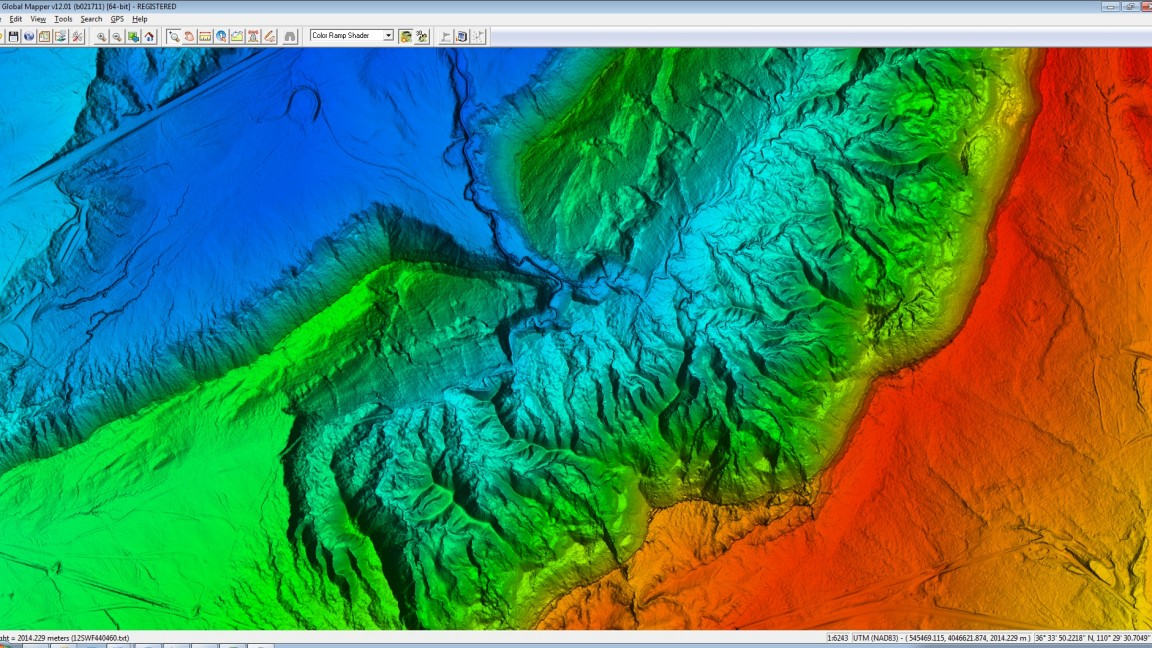
\includegraphics[width=\linewidth]{LIDAR.jpg}

\end{figure}
\subsection{Canopy Height Model}
\end{document}
